\chapter{Introduction}
\label{cap:intro}

\section{Problem Statement}

Skin cancer, including melanoma, represents a significant public health concern
worldwide. Melanoma, in particular, poses a considerable challenge due to its
high mortality rate and the need for early detection for successful treatment.
Early and correct diagnosis is key for ensuring patients have the best possible
prognosis. Melanoma misdiagnosis accounts for more pathology and dermatology
malpractice claims than any cancer other than breast cancer, as an early
misdiagnosis can significantly reduce a patient’s chances of survival
\cite{Melanoma}. \newline

Dermoscopy, also known as dermatoscopy \textit{Figure
\ref{fig:procedure_dermoscopy}}, is a noninvasive technique widely utilized for
the examination of cutaneous lesions. It involves the use of a handheld
instrument called a dermatoscope to visualize subsurface skin structures that
are typically not visible to the naked eye. The dermatoscope illuminates the
skin surface and provides magnification, allowing for a detailed examination of
the epidermis, the dermoepidermal junction, and the papillary dermis. By
analyzing these structures, dermatologists can identify specific features and
patterns associated with various skin conditions, including melanoma
\cite{Dermoscopy}.

\begin{figure}[htb] \centering
  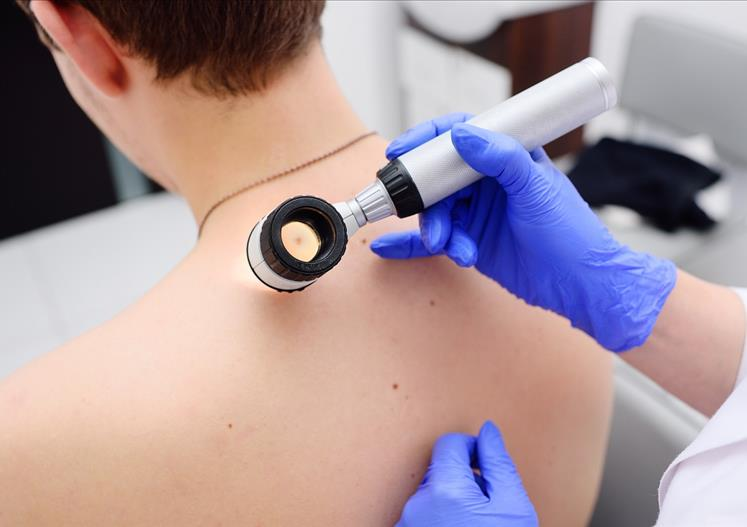
\includegraphics[width=6.5 cm]{imatges/introduction/medical_procedure_dermastocopy.jpeg}
  \caption[Dermoscopy Procedure]{\textit{During the dermoscopy procedure, the dermatologist places the dermatoscope directly on the skin, making contact with the lesion of interest. Illustration by MD Anderson Cancer Center}}
  {\label{fig:procedure_dermoscopy}}
\end{figure}

Worldwide, in 2020 an estimated 324,635 people were diagnosed with melanoma and
an estimated 57,043 people worldwide died from melanoma the same year
\cite{CancerStats}. The introduction of sophisticated machinery and techniques
in dermoscopy procedures \textit{Figure \ref{fig:subset_isic}} seems not enough
to fight against melanoma, but the developments in artificial intelligence (AI)
especially in deep learning techniques, have made Computer-Aided Diagnosis
(CAD)\footnote{Computer-Aided Diagnosis (CAD) refers to the use of computer
algorithms and technologies to assist healthcare professionals in the process
of medical diagnosis} a promising path towards medical automation.

\begin{figure}[h!] \centering
  \begin{subfigure}{0.3\textwidth}
    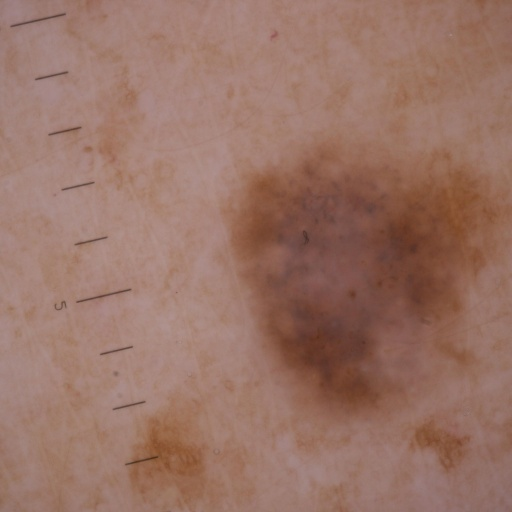
\includegraphics[width=\textwidth]{imatges/introduction/subset_isic/ISIC_1752943.jpg}
  \end{subfigure}
  \hfill
  \begin{subfigure}{0.3\textwidth}
    
\includegraphics[width=\textwidth]{imatges/introduction/subset_isic/ISIC_1766619.jpg}
  \end{subfigure}
  \hfill
  \begin{subfigure}{0.3\textwidth}
    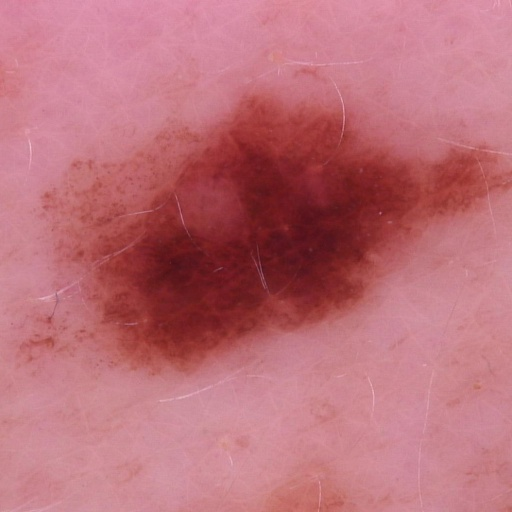
\includegraphics[width=\textwidth]{imatges/introduction/subset_isic/ISIC_1448526.jpg}
  \end{subfigure}
  \caption[Dermoscopy Images]{\textit{Dermoscopy Images. Illustration by ISIC Archive}}
  \label{fig:subset_isic}
\end{figure}

However, there are several limitations that raise doubts about the effectiveness of automated melanoma cancer classifiers and their suitability for integration into the medical system. Firstly, certain methods are constructed based on theoretical models of melanoma appearance, which may restrict their applicability to specific morphologies and fail to capture the wide range of variations seen in real-world scenarios. Secondly, AI systems utilized in these classifiers are trained to address a singular and narrow task. Unlike human dermatologists, these systems lack the ability to consider holistic patient information when formulating a final diagnosis, reflecting the concept of weak AI \cite{WeakAI}. Lastly, numerous methods have been trained and evaluated using high-quality image frames, which may result in instability when applied under real-time visibility conditions where image quality is often compromised. A fundamental part of machine learning is the problem of generalization, that
is, how to make sure that a trained model performs well on unseen data. If the
unseen data has different distribution, i.e. a domain shift exists, the problem
is significantly more difficult even the smallest changes in the statistics as
compared to the training data can cause a deep neural network to fail
completely \cite{DomainShift}. \newline

Addressing these limitations and developing melanoma cancer classifiers that
encompass a wider range of morphologies, incorporate holistic patient
information, consider relevant elements, and demonstrate robustness in
real-world scenarios are crucial for improving the reliability and
effectiveness of melanoma detection and diagnosis systems. \newline

\section{Project Objectives}

The main objective of this project is to create a health care infrastructure,
focused on melanoma detection using deep learning methods to train a system
capable of detecting melanoma on dermoscopy images to test the ability of
computer-assisted image analysis. To this end, the gradual achievements that
must be accomplished are:

\begin{itemize}
  \item Gaining a comprehensive understanding of the theory behind deep learning and its practical applications.
  \item Analyzing images from dermostocopy and understanding its most important features.
  \item Train deep learning models with different techniques based on tranfer-learning focused on the images of the melanoma ISIC Challenge \cite{IsicChallenge}.
  \item Developing a CAD infrastructure. The CAD infrastructure contains the already trained models with a simple web UI\footnote{The user interface (UI) is the point of human-computer interaction and communication in a device} an API\footnote{API stands for Application Programming Interface} and finally a mechanism using Docker to virtualize this services making it ease to deploy in any based Linux System.
\end{itemize}

\section{Personal Motivation}

I envisioned this project as a unique fusion of three personal passions.
Firstly, I was fueled by a deep fascination with human cognition and reasoning.
Machines, in my eyes, represented a novel paradigm through which I could delve
further into this captivating realm. \newline

I am also motivated by the remarkable problem-solving capacity of data.
Regardless of its structure, data holds immense potential to uncover hidden
patterns, provide insights, and drive innovation. The ability to extract
meaningful information from data, regardless of its form, inspires me to
constantly expand my knowledge and skills in order to contribute to the field
of data science and make a tangible difference in the world. \newline

Last but not least, I am driven by the immense power of automation and its
ability to democratize access to research knowledge. I am amazed by how
automation processes can extract value and make them readily available to
professionals and the public alike.

\section{Statement of Originality}

I, Wilber Eduardo Bermeo Quito, declare that the thesis titled "A Platform for
Classifying Melanoma" is an original work completed with the support and
collaboration of Accenture SL and the VICOROB laboratory. \newline

The content presented in this thesis is the outcome of my independent research
efforts, guided by the knowledge and expertise acquired through my academic
studies and the valuable contributions from Accenture S.L and the VICOROB
laboratory. \newline

I acknowledge the importance of academic integrity and the consequences of
plagiarism. Hence, I affirm that all the information, data, results, figures,
and conclusions presented in this thesis are authentic and original. Any
references or sources used have been appropriately cited and referenced.

\section{Regulatory Framework}

The inclusion of legal considerations has become a significant aspect of the
field of medical imaging. Privacy concerns and the potential misuse of personal
information make sharing and distributing medical data particularly
challenging. To address these limitations, recent research collaborations have
focused on promoting the sharing of patient data through de-identification
methods. However, it is crucial to thoroughly analyze the obligations related
to the protection of individuals and their personal data before engaging in
projects involving medical imaging. \newline

When working with medical images, it is the utmost importance to prioritize
patient privacy rights. In the context of developing a skin lesions database,
it is necessary to obtain signed consent from patients for the publication of
their data. For this thesis, the ISIC Archive database was utilized, this
database serves as a publicly accessible resource for teaching, research, and
the development and testing of diagnostic artificial intelligence algorithms,
and it resolves any concerns related to consent \cite{IsicArchive}. It is a
large and continually expanding open-source archive of skin images.

\section{Related Work}

Melanoma Computer-Aided Diagnosis (CAD) classifiers have been a subject of extensive research and development in recent years,
also there has been a lot of work in platforms capable of explaining the way
these models infer. Bellow is mentioned remarkable related work to the subject.
\newline

\vspace{0.5cm}
\textbf{Identifying Melanoma Images using EfficientNet Ensemble: Winning Solution to the SIIM-ISIC Melanoma Classification Challenge} \newline

Winning solution to the SIIM-ISIC Melanoma Classification Challenge. It is an
ensemble of convolutions of neural network (CNN) models with different
backbones and input sizes \cite{WinningISIC}.  \newline

\vspace{0.5cm} \textbf{Dermatologist-level classification of skin cancer with
deep neural networks} \newline

This study demonstrated the use of a deep learning algorithm to classify skin
lesions, including melanoma, with accuracy comparable to dermatologists. The
deep neural network was trained on a large dataset of images and achieved high
sensitivity and specificity \cite{SkinCancerDeepNN}. \newline

\vspace{0.5cm} \textbf{Computerized analysis of pigmented skin lesions: A
review}  \newline

The goal of this paper is to give a detailed explanation and clear up any
confusion about the words and phrases used in melanoma studies. And to organize
and group together useful sources, making it easier to find information on a
particular sub-topic when searching through the existing literature
\cite{MelanomaTopicsReview}. \newline

\newpage

\vspace{0.5cm}
\textbf{CNN-Explainer} \newline

The CNN-Explainer is an interactive web-based tool that aims to provide
explanations for the predictions made by convolutional neural network (CNN)
models \cite{CNNExplainer}.

\section{Contribution to Melanoma Detection}

In this section, we present the contribution to the field of melanoma detection
through the development of a melanoma CAD (Computer-Aided Diagnosis)
infrastructure classifier. \newline

The thesis comprises multiple models employing various techniques, including
transfer learning, data augmentation, just-in-time testing, regularization, and
others. To compare these models, tools like W\&B (Weight \& Biases), a MLOps
platform for experiment tracking, and MLXTEND, providing utilities and
extensions for machine learning and data science in Python's scientific
computing stack, were utilized. The experiments were conducted using the ISIC
Archive dataset, consisting of benign and malignant skin lesions. Prior to
analysis, the dataset underwent preprocessing to enhance quality and normalize
features. Consequently, accurate classification and differentiation of melanoma
lesions from benign ones were achieved. \newline

In order to to ensure the usability of the trained models,
two services were developed. These services include a user-friendly UI and an
API, both of which were containerized using Docker technology. By
containerizing the UI, an intuitive and interactive user experience was
provided, enabling users to seamlessly interact with the melanoma CAD system.
Similarly, containerizing the API streamlined request handling and prediction
serving, resulting in efficient performance. This approach facilitated easy
deployment across various platforms.
